
\section{Force, Mass and Acceleration\footnote{
1990-93 Dept. of Physics and Astronomy, Dickinson College. Supported by FIPSE
(U.S. Dept. of Ed.) and NSF. Portions of this material may have been modified
locally and may not have been classroom tested at Dickinson College.
}}

\makelabheader %(Space for student name, etc., defined in master.tex or labmanual_formatting_commands.tex)

\bigskip
\textbf{Objectives }

\begin{itemize}
\item To develop a definition of mass in terms of an object's motion under the influence
of a force. 
\item To understand the relationship among the force applied to an object, the mass
of the object and its motion. 
\item To find a mathematical relationship between the acceleration of an object and
its mass when a constant force is applied--Newton's Second Law. 
\item To examine the quantitative relationship between force, mass and acceleration--Newton's
Second Law--in terms of the SI units (N for force, kg for mass, and (m/s)/s for
acceleration). 
\item To pull all of the observations together and state Newton's First and Second
Laws of Motion for motion in one dimension, along a straight line for any number
of forces acting on an object.
\end{itemize}

\bigskip
\textbf{Apparatus }

\begin{itemize}
\item Force probe 
\item Motion detector 
\item Dynamics cart and track 
\item Variety of masses to increase the mass of the cart 
\item CS2000 compact scale
\item Low friction pulley and string 
\item Variety of hanging masses 
\item \textit{Science Workshop 750 Interface }
\item \textit{DataStudio} software (V, A \& F Graphs)
\end{itemize}

\bigskip
\textbf{Overview }
\medskip

In this lab you will continue to develop the first two of Newton's famous laws
of motion. You will do this by combining careful definitions of force and mass
with observations of the mathematical relationships among force, mass and acceleration.
\medskip

You have seen that the acceleration of an object is directly proportional to
the combined or net force acting on the object. If the combined force is not
zero, then the object will accelerate. If the combined force is constant, then
the acceleration is also constant. These observations are part of Newton's Second
Law of Motion.
\medskip

You have also seen that for an object to move at a constant velocity (zero acceleration)
when friction is negligible, the combined or net force on the object should
be zero. The law which describes constant velocity motion of an object is Newton's
First Law of Motion. Newton's First and Second Laws of Motion are very powerful!
They allow you to relate the force on an object to its subsequent motion. Therefore,
when the nature of the force(s) acting on an object is known, then Newton's
laws of motion allow you to make mathematical predictions of the object's motion. 

In the first part of this lab you will study how the amount of ``stuff''
(mass) you are accelerating with a force affects the magnitude of the acceleration.
What if the mass of the object were larger or smaller? How would this affect
the acceleration of the object for a given combined force? 

In the second part you will study more carefully the definitions of the units
in which we express force, mass and acceleration.

Finally, in the last part, you will examine the motion of an object caused by
a force applied to it when friction is large enough so that it cannot be ignored.
\medskip

\textbf{Force, Mass and Acceleration }

In previous activities you have applied forces to a cart and examined its motion.
Up until now, you have always used a cart with the same mass. But when you apply
a force to an object, you know that its mass has a large effect on the object's
acceleration. For example, compare the different accelerations that would result
if you pushed a 1000 kilogram (metric ton) automobile and a 1 kilogram cart,
both with the same size force! 

\medskip
\textbf{Activity 1: Acceleration and Mass }

You can easily change the mass of the cart by attaching masses to it, and you
can apply the same force to the cart by using appropriate hanging masses to
accelerate the cart each time. By measuring the acceleration of different mass
carts, you can find a mathematical relationship between the acceleration of
the cart and its mass, with the applied force kept constant.

(a) Calibrate the force probe (see \textit{Calibrating Force Sensors} in \textbf{Appendix \ref{capstone}: Capstone}).
\medskip

(b) Set up the pulley, cart, string, motion detector and force probe as shown
below. (Be sure that the cable from the force probe doesn't interfere with the
motion of the cart, and is out of the way of the motion detector.)
\bigskip

\vspace{0.3cm}
{\par\centering 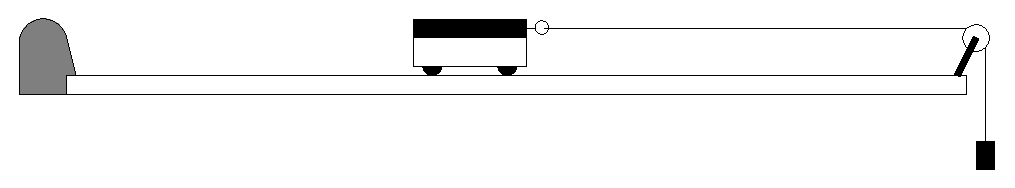
\includegraphics{force1/force1_fig4.eps} \par}
\vspace{0.5cm}

(c) We will define a mass scale in which the unit is the mass of the cart (including the force probe), called one cart mass. Use the compact scale to determine the mass of the cart and force probe. This will be defined as one cart mass. Assemble masses which you can add to the cart to make the cart's mass equal to approximately 1.5, 2.0. 2.5 and 3.0 cart masses. Record the amount of mass to be added in each case.
\medskip

(d) Now add masses to make the cart's mass 2.0 cart masses.
\medskip

(e) Hang 100 g from the end of the string.
Start recording data and release the car from rest when you hear the clicks
of the motion detector. Repeat until you get a good run. Sketch the graphs on
the axes below. Don't forget to label the axes.

\pagebreak[2]
\answerspace{0.3cm}
{\par\centering 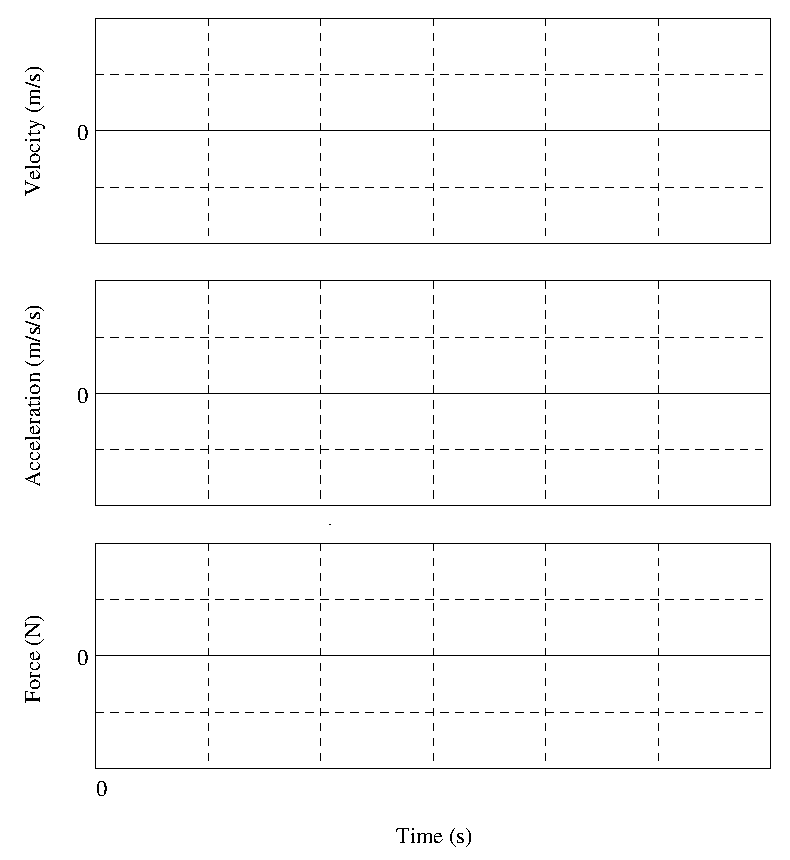
\includegraphics{force2/force2_fig4.eps} \par}
\answerspace{0.3cm}

(f) Use the Smart Tool to determine the average force and average acceleration
during the time interval when they are nearly constant, and record them in the
third row of the table below.

\vspace{0.3cm}
{\centering \begin{tabular}{|c|c|c|}
\hline 
Mass of Cart&
Average Applied&
Average Acceleration\\
(cart masses)&
Force (N)&
(m/s\( ^{2} \))\\
\hline 
\hline 
1.0&
&
\\
&
&
\\
\hline 
1.5&
&
\\
&
&
\\
\hline 
2.0&
&
\\
&
&
\\
\hline 
2.5&
&
\\
&
&
\\
\hline 
3.0&
&
\\
&
&
\\
\hline 
\end{tabular}\par}
\answerspace{0.3cm}

\pagebreak[2]
(g) Suppose that you halve the mass of the cart back to 1.0 cart masses, and
accelerate it with the same applied force. How would the acceleration compare
with that of the 2.0 cart masses?
\answerspace{20mm}

(h) Test your prediction. Remove the masses you added earlier which doubled
the mass of the cart to 2.0 cart masses. 

\textbf{Comment:} You want to accelerate the cart with the same applied force.
As you may have noticed, the force applied to the force probe by the string
decreases once the cart is released. (You will examine why this is so in a later
lab.) This decrease depends on the size of the acceleration. Therefore, in order
to keep the applied force constant, you may need to change the hanging mass. 

Adjust the hanging mass until the force probe reading while the cart is accelerating
is the same as the force you recorded in the third row of the table above. When
you have found the correct hanging mass, graph the motion of the cart. Measure
the average force and average acceleration of the cart during the time interval
when the force and acceleration are nearly constant and record these values
in the first row of the table.

(i) Did the acceleration agree with your prediction? Explain.
\answerspace{20mm}

(j) Now make the mass of the cart 1.5 cart masses, and accelerate it again with
the same size force. (Don't forget to adjust the hanging mass, if necessary.)
Measure the average force and acceleration of the cart, and record these values
in the table. Repeat for masses of 2.5 and 3.0 cart masses.

(k) Does the acceleration of the cart increase, decrease or remain the same
as the mass of the cart is increased?
\answerspace{10mm}

(l) Use Excel to plot the acceleration (y axis) as a function of the
cart mass (x axis) and to find the best fit to the data. When you have found
the best fit, print the graph and put a copy in your notebook. 

(m) What appears to be the relationship between acceleration and mass of the
cart, when the applied force is kept constant?
\answerspace{20mm}

(n) In the previous lab, you found that the acceleration of the cart was proportional
to the combined applied force, when the mass of the cart was not changed. State
in words the general relationship between the applied force, the mass and the
acceleration of the cart which you have found in these two labs. If the combined
force is \( \sum{\bf F}  \), the mass is m and the acceleration is a,
write a mathematical relationship which relates these three physical quantities.
\answerspace{20mm}

\pagebreak[2]
\textbf{Force \& Mass Units} 

So far you have been measuring force in standard units called newtons. Where
does this unit come from? By contrast, we have our own private units for mass,
measuring mass in cart masses. If one group were using a large wooden cart in
their force and motion experiments, and another group were using a small aluminum
cart with smaller mass, they would have different values for mass, and would
observe different accelerations for ``one cart mass pulled by one newton.''
It's time to discuss standard units for force and mass.

It would be nice to be able to do a mechanics experiment in one part of the
world and have scientists in another part of the world be able to replicate
it or at least understand what actually happened. This requires that people
agree on standard units. In 1960 an international commission met to agree upon
units for fundamental quantities such as length, time, mass, force, electric
current, pressure, etc. This commission agreed that the most fundamental units
in the study of mechanics are length, time, and mass. All other units including
force, work, energy, torque, rotational velocity, etc. which you encounter in
your study of mechanics can be expressed as a combination of these basic quantities.
The fundamental International System or SI units along with the standard unit
for force are shown below.

\textbf{Fundamental Units for Mechanics }

Length: A \textbf{meter (m)} is the distance traveled by light in a vacuum during
a time of 1/299,792,458 second. 

Time: A \textbf{second (s)} is defined as the time required for a cesium-133
atom to undergo 9,192,631,770 vibrations. 

Mass: A \textbf{kilogram (kg)} is defined as the mass of a platinum-iridium
alloy cylinder kept at the International Bureau of Weights and Measures in S�vres
France. It is kept in a special chamber to prevent corrosion.

\textbf{The Force Unit Expressed in Terms of Length, Mass, and Time} 

Force: A newton (N) is defined as that force which causes a 1 kg mass to accelerate
at 1 (m/s)/s . 

We want to be able to measure masses in kilograms and forces in newtons in our
own laboratory. The following activities are designed to give you a feel for
standard mass and force units, and how they are determined in the laboratory.
Our approach in these activities is to use a standard force scale to calibrate
the force probe in newtons. Using your data from the previous investigation,
you will see how you can establish a mass unit in terms of your force and acceleration
measurements. Then you will use a standard mass scale to get enough stuff loaded
on a cart to equal one kilogram of mass. Finally you can pull the cart with
a force of about one newton and see if it accelerates at something close to
one meter per second per second. \textbf{Warning:} There will probably be a
noticeable amount of uncertainty associated with the necessary measurements.

Suppose you want to find the mass of an object in kilograms. You need to compare
it to the one kilogram platinum-iridium alloy cylinders at the International
Bureau of Weights and Measures in France. It would be nice to have a standard
kilogram in your laboratory. You could go to France, but it is unlikely that
they would let you take the standard home with you!

Suppose, however, that you accelerate the standard mass with a constant force
and measure the force and also the resulting acceleration as accurately as possible.
Next you would need to make a cylinder that seemed just like the standard one
and add or subtract stuff from it until it undergoes exactly the same acceleration
with the same constant force. Then within the limits of experimental uncertainty
this new cylinder standard and the bureau standard would have the same mass.
If the comparison could be made to three significant figures, then the mass
of your new standard would be \( m_{std}  = 1.00\) kg.

Suppose you head home with your standard mass. You wish to determine the mass
of another object. You could apply the same constant force, F, on the standard
and on the other object, and measure both accelerations. Then, according to
Newton's Second Law, F = ma,
\[
m_{\rm std}=1.00\: {\rm kg}=\frac{F}{a}\qquad m_{\rm other}=
\frac{F}{a_{\rm other}}\]

\vspace{-0.2cm}
Since the constant force, F, applied to both masses was the same,
\[
m_{\rm other}=1.00\: {\rm kg}\: \frac{a}{a_{\rm other}}\]


In fact, you have already done something similar in the last investigation. 

\pagebreak[2]
\textbf{Activity 2: Calculating One ``cart mass'' in Standard
Units }

(a) In Activity 1, you measured the force applied to a cart and the acceleration
of the cart with 1.0, 1.5, 2.0, 2.5 and 3.0 cart masses. Turn back to your table
of information from that experiment, and copy the values of average force and
average acceleration into the second and third columns of the table below.

\vspace{0.3cm}
{\centering \begin{tabular}{|c|c|c|c|c|}
\hline 
Mass of Cart&
Average Applied&
Average Acceleration&
Ratio of F/a&
Mass of cart\\
(cart masses)&
Force (N)&
(m/s\( ^{2} \))&
(calculated mass)&
from scale (kg)\\
\hline 
\hline 
1.0&
&
&
&
\\
&
&
&
&
\\
\hline 
1.5&
&
&
&
\\
&
&
&
&
\\
\hline 
2.0&
&
&
&
\\
&
&
&
&
\\
\hline 
2.5&
&
&
&
\\
&
&
&
&
\\
\hline 
3.0&
&
&
&
\\
&
&
&
&
\\
\hline 
\end{tabular}\par}
\vspace{0.3cm}

In the discussion above, the mass in standard units was calculated using Newton's
second law by taking the ratio of the combined (net) force on the object in
newtons to the acceleration of the object measured in meters per second per
second. (b) For each row in the table, calculate the ratio of the force to acceleration
and record it in the fourth column.

(c) According to the discussion, the values you just calculated should be the
mass of the object in kilograms. Do your numbers seem to make sense? What do
you get for the value of 1.00 cart mass in kilograms (from column 4 above)? What do you get for the value of 2.00 cart masses in kilograms?
\answerspace{15mm}

\textbf{Comment:} Physicists call the quantity you have just calculated--the
ratio of combined (net) force on an object to its acceleration--the inertial
mass of the object. You could continue to determine and compare masses by accelerating them and taking force to acceleration ratios, but this process is pretty tedious.
A simpler approach is to use an electronic scale or a mechanical balance that
has already been calibrated in kilograms using a standard mass by somebody who
is intelligent and knowledgeable! (The details of why such devices can give
us correct masses in kg will not be easy to understand fully until after gravitational forces are studied.) 

(d) Compare your inertial mass calculations for 1.0, 1.5, 2.0, 2.5 and 3.0 cart
masses (fourth column above) with the values you get by adding the amounts recorded in Activity 1(c) to the value you measured for one cart mass in Activity 1(c). Record these values in the last column of the table.

(e) Are your inertial masses reasonably consistent with your scale masses?
\answerspace{10mm}

(f) Plot average acceleration (column 3 above) vs mass of cart (column 5 above) as a power function (using \textit{Excel}). Does the resulting power make sense?
\answerspace{5mm}

\textbf{Comment:} In your experiments, you have seen that the physical quantities
force, mass and acceleration are related through Newton's Second Law. In the
activity you have just done, you have used this relationship to define inertial
mass in terms of standard units of force, length and time. This is a good logical
definition of inertial mass. Historically, however, the units of mass, length
and time were defined first as standards and the unit of force was defined as
a derived unit in terms of these standard units. Thus a newton of force is defined
as the force needed to accelerate 1.00 kg at 1.00 (m/s)/s. In the next activity
you will examine this definition. 

\pagebreak[2]
\textbf{Activity 3: Does a Force of 1.0 N Applied to a 1.0 kg Mass Really Cause
an Acceleration of 1.0 meter/second/second?} 

You have used mass and force measuring devices that have been provided for you.
You could now see if everything makes sense by accelerating one kilogram of
mass with a force of about one newton and seeing if an acceleration of about
one meter per second per second results. Unfortunately, the carts with force
probes that we have been using typically have a mass greater than 1 kg. So we
will accelerate a 2.0 kg cart with a 2.0 N force.

(a) What do you expect the acceleration to be in this case? Show the calculation
below.
\vspace{20mm}

(b) Test your prediction. Add masses to the cart so that the total mass is 2.0
kg. Set up the pulley, weighted cart, string, motion detector and force probe
as in Activity 1. Check the calibration of the force probe with a force of 2.0
N (hanging mass of 200 g). Graph the motion and measure the acceleration that
results from an applied force on the force probe of 2 N. Adjust the hanging
mass, if necessary, to get an applied force of close to 2 N while the cart is
accelerating. (Comment: Be careful! Remember that when the cart is being held
at rest the same hanging mass will exert more applied force on the cart than
when it is accelerating.) Once you get a good run, measure the average values
of force and acceleration, and record these values in a table below. Also record
the mass of the cart and the hanging mass.
\vspace{30mm}

(c) How close is your result to the expected value of acceleration? Calculate
the \% difference.
\vspace{20mm}

(d) A force of 5.4 N is applied to an object, and the object is observed to
accelerate with an acceleration of 3.0 (m/s)/s. If friction is so small that it
can be ignored, what is the mass of the object in kg? Show your calculation.
\vspace{20mm}

(e) An object of mass 39 kg is observed to accelerate with an acceleration of
2.0 (m/s)/s. If friction is negligible, what is the force applied to the object
in N? Show your calculation.
\vspace{20mm}

\textbf{Comment:} The main purpose of the last three labs has been to explore
the relationship between the forces on an object, the object's mass, and its
acceleration. You have been trying to develop Newton's First and Second Laws
of Motion for one-dimensional situations in which all forces lie in a positive
or negative direction along the same line. 

\pagebreak[2]
\textbf{Activity 4: Newton's Laws in Your Own Words} 

(a) Express Newton's First Law (the one about constant velocity) in terms of
the combined (net) force applied to an object in your own words clearly and
precisely.
\vspace{20mm}

(b) Express Newton's First Law in equations in terms of the acceleration vector,
the combined (net) force vector applied to an object, and its mass.
\[
\mbox{If}\; \sum {\bf F}= \qquad \mbox{then}\; {\bf a}=
\qquad \mbox{and}\; {\bf v}=\]


(c) Express Newton's Second Law (the one relating force, mass, and acceleration)
in terms of the combined (net) force applied to an object in your own words
clearly and precisely.
\vspace{20mm}

(d) Express Newton's Second Law in equations in terms of the acceleration vector,
the combined (net) force vector applied to an object, and its mass.
\[
\mbox{If}\; \sum {\bf F}\neq 0\qquad \mbox{then}\; 
{\bf a}=\]


\textbf{Homework} 

Questions 1 and 2 refer to a toy car which can move in either direction along
a horizontal line (the + position axis).

%\vspace{0.3cm}
{\par\centering 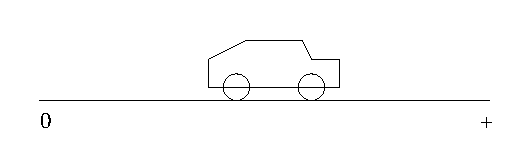
\includegraphics{force2/force2_fig6.eps} \par}
%\vspace{0.3cm}

Assume that friction is so small that it can be ignored. A force toward the
right of constant magnitude is applied to the car. 

1. Sketch on the axes below using a solid line the shape of the acceleration-time
graph of the car.

%\vspace{0.3cm}
{\par\centering 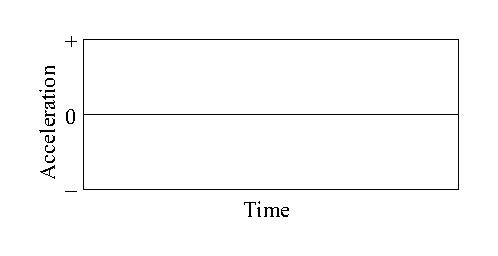
\includegraphics{force_mass/force_mass_fig1.eps} \par}
%\vspace{0.3cm}

2. Suppose that the mass of the car were twice as large. The same constant force
is applied to the car. Sketch on the axes above using a dashed line the acceleration-time
graph of the car. Explain any differences in this graph compared to the acceleration-time
graph of the car with the original mass.
\answerspace{10mm}

\pagebreak[2]
3. When a force is applied to an object with mass equal to the standard kilogram,
the acceleration of the mass is 3.30 (m/s)/s. (Assume that friction is so small
that it can be ignored.) When the same magnitude force is applied to another
object, the acceleration is 2.20 (m/s)/s. What is the mass of this object? What
would the object's acceleration be if a force twice as large were applied to
it? Show your calculations.
\answerspace{20mm}

4. Given an object with mass equal to the standard kilogram, how would you determine
if a force applied to it has magnitude just equal to one newton? (Assume that
friction is so small that it can be ignored.)
\answerspace{20mm}

5. The spring scale in the diagram below reads 10.5 N. (Assume that friction
is so small that it can be ignored.)

%\vspace{0.3cm}
{\par\centering 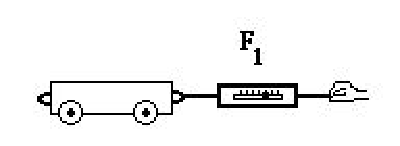
\includegraphics{combining/combining_fig2.eps} \par}
%\vspace{0.3cm}

If the cart moves toward the right with an acceleration toward the right of
3.50 (m/s)/s, what is the mass of the cart? Show your calculations and explain.
\answerspace{20mm}

6. The force applied to the cart in (5) by spring scale \( F_{1} \) is still
10.5 N. The cart now moves toward the right with a constant velocity. What are
the magnitude and direction of the frictional force. Show your calculations
and explain. (Assume that friction can not be ignored.)
\answerspace{20mm}

7. The force applied to the cart in (5) by spring scale \( F_{1} \) is still
10.5 N. The cart now moves toward the right with an acceleration toward the
right of 1.75 (m/s)/s. What are the magnitude and direction of the frictional
force. Show your calculations and explain.
\answerspace{20mm}

8. The force applied to the cart by spring scale \( F_{1} \) is 10.5 N.

%\vspace{0.3cm}
{\par\centering 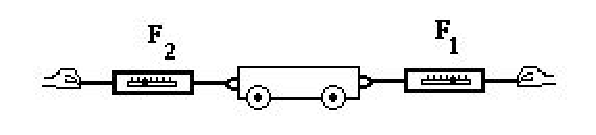
\includegraphics{combining/combining_fig4.eps} \par}
%\vspace{0.3cm}

The cart now moves toward the right with a constant velocity. The frictional
force has the same magnitude as in (7). What does spring scale \( F_{2} \)
read? Show your calculations and explain.

